\documentclass{ddis-thesis}
\usepackage{amsmath, amsthm, amssymb}
\usepackage[latin1]{inputenc}
\usepackage{program}
\usepackage{mathrsfs}
\usepackage{amsfonts}

\usepackage{fancyvrb}
\DefineVerbatimEnvironment{code}{Verbatim}{fontsize=\small}
\DefineVerbatimEnvironment{example}{Verbatim}{fontsize=\small}


\usepackage{fancyhdr}% fancyhdr related command; details in its documentation
\pagestyle{fancy}
\fancyhead{}
\fancyhead[LE,RO]{\thepage}
\fancyhead[RE]{\leftmark}
\fancyhead[LO]{\rightmark}


\usepackage{graphicx}
\author{name}
\title{Thesis title}
\begin{document}

% *************** Front matter ***************

\frontmatter
\begin{titlepage}

\setlength{\textwidth}{16cm}
\setlength{\oddsidemargin}{0cm}
\setlength{\evensidemargin}{0cm}
\setlength{\topmargin}{8mm}
\setlength{\headheight}{0cm}
\setlength{\headsep}{0cm}
\setlength{\topskip}{0cm}
\enlargethispage{5cm}

\noindent
\setlength{\unitlength}{1mm}

\begin{picture}(160,226)
\centering

\put(0,203){\line(1,0){160}} % lower line
\put(109,39){\line(1,0){50}}
\put(109,161){\line(1,0){50}}
\put(109,170){\line(1,0){50}}
\put(107,1){\line(0,1){200}}

\put(0,140){\parbox[b]{100mm}{
    \begin{center}
    {\bf\Huge {\sffamily{Thesis Title}}}
    \end{center}}}


\put(109,92){\parbox[b]{50mm}{
    {\bf
    {\sffamily{{\Large Imaginary Student}}}}\\
    {\sffamily{of Basel BS, Switzerland\\\\
    Student-ID: 00-000-000\\
    img\_student@gmx.net
    }}
}}

\put(109,161){\makebox(50,9){{\sffamily{Thesis \hfill\today}}}}

\put(0,215){\makebox(80,11)[l]{
\includegraphics[height=2.8cm]
{./section-title/figures/uzh_logo_e_pos}}}


\put(109,32){\parbox[b]{50mm}{\flushleft
    {\sffamily{Advisor:}} {\bf {\sffamily{Advisor Name}} }
    }
}

\put(109,10){\parbox[b]{50mm}{\flushleft
        {\sffamily{
        Prof. Abraham Bernstein, PhD\\
        Institut f\"ur Informatik\\
        Universit\"at Z\"urich\\
        http://www.ifi.uzh.ch/ddis}
        }
}}

\end{picture}
\end{titlepage}



\begin{acknowledgements}
Lorem ipsum dolor sit amet, consectetuer adipiscing elit. Nullam a tellus.
Aliquam commodo dui non ipsum. Duis mollis nisi id turpis. Donec quis ipsum.
Curabitur sed nibh. Morbi suscipit justo quis orci. Ut massa tortor, ultricies
vitae, lacinia eu, facilisis eu, nisl. Nulla mattis urna sed metus imperdiet
ornare. Praesent sodales. Etiam laoreet. Mauris quam magna, sagittis et,
pharetra eget, congue vitae, arcu. Fusce sollicitudin justo. Suspendisse
lectus. Sed lobortis dolor quis lectus scelerisque ornare. Integer purus.
Phasellus vel elit at nibh sagittis lobortis. Aliquam iaculis malesuada eros.
Mauris metus.
\end{acknowledgements}

\begin{zusammenfassung}
Lorem ipsum dolor sit amet, consectetuer adipiscing elit. Nullam a tellus.
Aliquam commodo dui non ipsum. Duis mollis nisi id turpis. Donec quis ipsum.
Curabitur sed nibh. Morbi suscipit justo quis orci. Ut massa tortor, ultricies
vitae, lacinia eu, facilisis eu, nisl. Nulla mattis urna sed metus imperdiet
ornare. Praesent sodales. Etiam laoreet. Mauris quam magna, sagittis et,
pharetra eget, congue vitae, arcu. Fusce sollicitudin justo. Suspendisse
lectus. Sed lobortis dolor quis lectus scelerisque ornare. Integer purus.
Phasellus vel elit at nibh sagittis lobortis. Aliquam iaculis malesuada eros.
Mauris metus
\end{zusammenfassung}

\begin{abstract}
Lorem ipsum dolor sit amet, consectetuer adipiscing elit. Nullam a tellus.
Aliquam commodo dui non ipsum. Duis mollis nisi id turpis. Donec quis ipsum.
Curabitur sed nibh. Morbi suscipit justo quis orci. Ut massa tortor, ultricies
vitae, lacinia eu, facilisis eu, nisl. Nulla mattis urna sed metus imperdiet
ornare. Praesent sodales. Etiam laoreet. Mauris quam magna, sagittis et,
pharetra eget, congue vitae, arcu. Fusce sollicitudin justo. Suspendisse
lectus. Sed lobortis dolor quis lectus scelerisque ornare. Integer purus.
Phasellus vel elit at nibh sagittis lobortis. Aliquam iaculis malesuada eros.
Mauris metus.
\end{abstract}


\tableofcontents

% *************** Main matter ***************
\mainmatter

\chapter{Introduction}
\label{k:einleitung} Lorem ipsum dolor sit amet, consectetuer adipiscing elit.
Nullam a tellus. Aliquam commodo dui non ipsum. Duis mollis nisi id turpis.
Donec quis ipsum. Curabitur sed nibh. Morbi suscipit justo quis orci. Ut massa
tortor, ultricies vitae, lacinia eu, facilisis eu, nisl. Nulla mattis urna sed
metus imperdiet ornare. Praesent sodales. Etiam laoreet. Mauris quam magna,
sagittis et, pharetra eget, congue vitae, arcu. Fusce sollicitudin justo.
Suspendisse lectus. Sed lobortis dolor quis lectus scelerisque ornare. Integer
purus. Phasellus vel elit at nibh sagittis lobortis. Aliquam iaculis malesuada
eros. Mauris metus.

Figure environment.

\begin{figure}
\centering
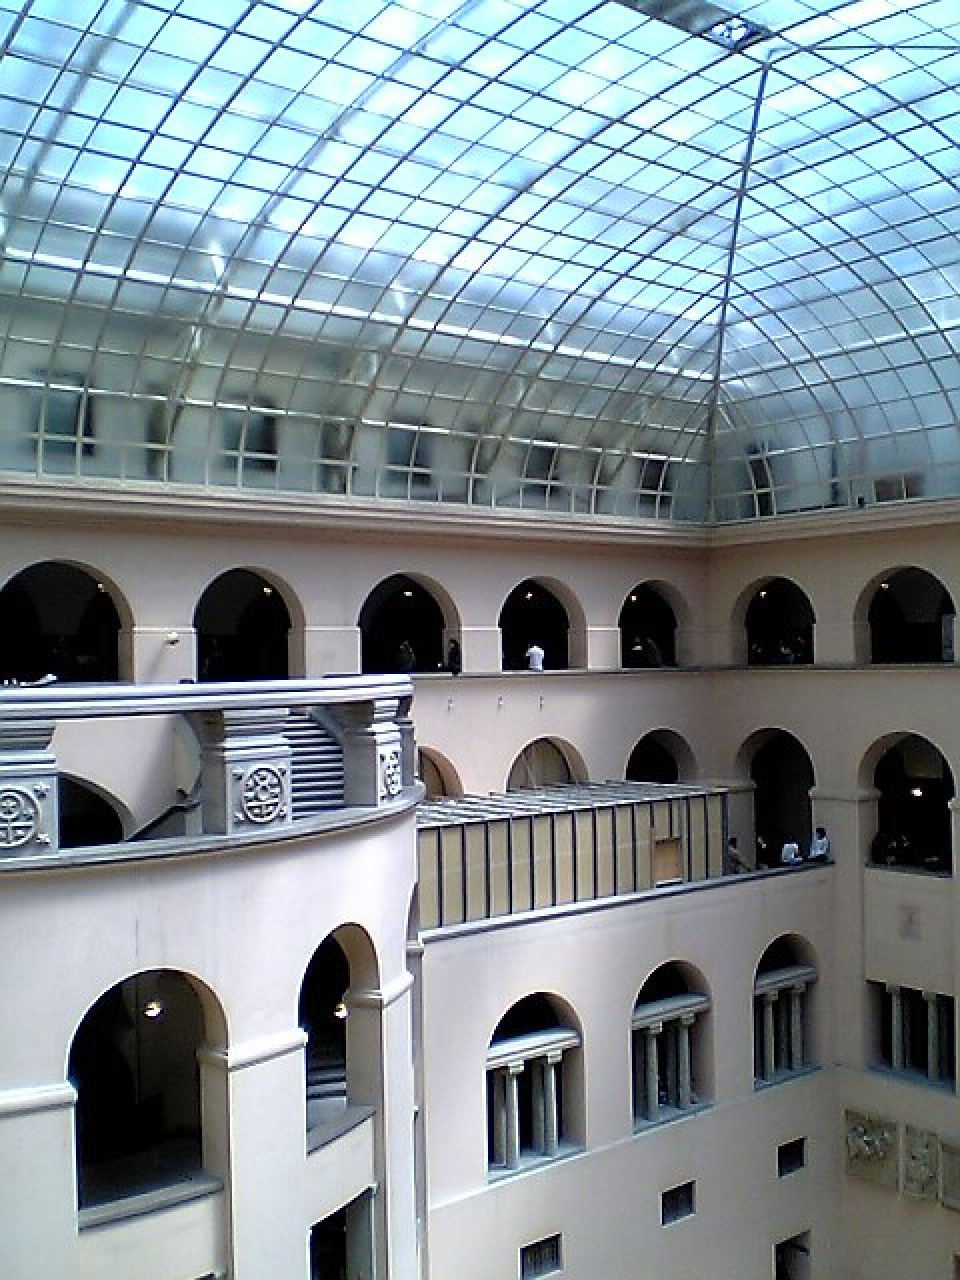
\includegraphics[height=2.0in,width=5.0in]{./section-introduction/figures/uzhlichthof.jpg}
\caption{image1 caption}
\label{f:figtag}
\end{figure}



In tellus mauris, nonummy eget, vestibulum in, interdum at, nulla. Vestibulum
eu justo. Vivamus lobortis pellentesque arcu. Aliquam enim risus, pulvinar
quis, pulvinar tempor, pharetra vitae, dolor. Aliquam ac sapien. Aenean augue
eros, malesuada nec, tincidunt eget, aliquet bibendum, odio. Maecenas eu est eu
nisi pulvinar bibendum. Lorem ipsum dolor sit amet, consectetuer adipiscing
elit. Pellentesque eleifend varius enim. Ut pharetra diam ac nulla. Aliquam a
turpis ac mi semper porttitor. Vivamus sodales molestie nibh. Vivamus in sapien
sit amet mauris sagittis lobortis. Aenean pretium. Suspendisse eu leo at quam
vehicula aliquam. Nunc a ipsum. Sed placerat fringilla nibh. Aliquam sagittis.
Integer a augue vitae libero elementum pretium. Proin metus (refer to Figure
\ref{f:fig1}) \cite{salton83introduction}.

Figure environment.

\begin{figure}[!ht]
\centering
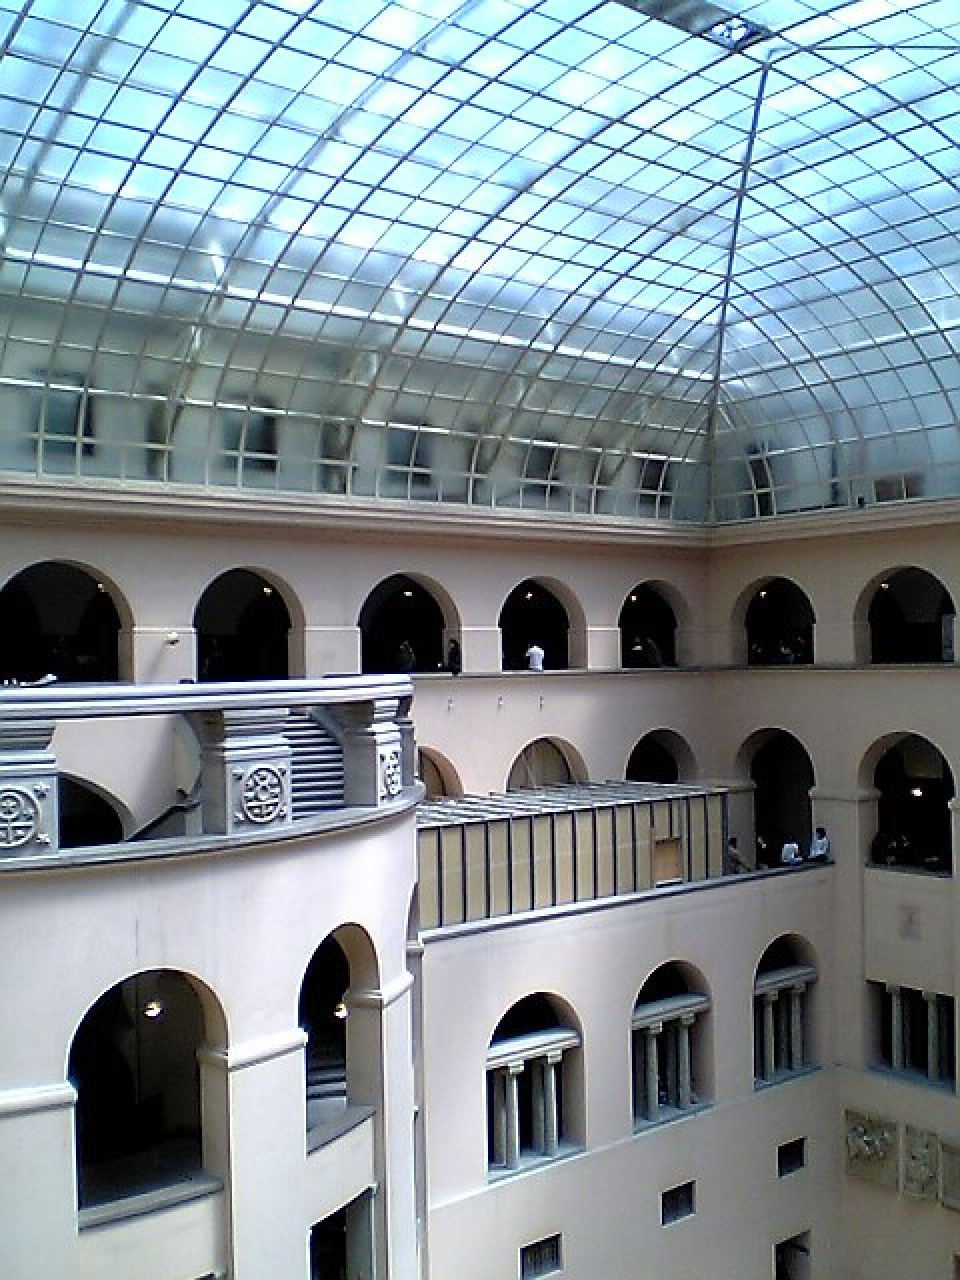
\includegraphics[width=\linewidth]{./section-introduction/figures/uzhlichthof.jpg}
\caption[Graphikbeschriftung MNO]{Graphic description UVW}
\label{f:fig1}
\end{figure}

\chapter{The First Chapter Title}
\label{c:chapter1} Lorem ipsum dolor sit amet, consectetuer adipiscing elit.
Nullam a tellus. Aliquam commodo dui non ipsum. Duis mollis nisi id turpis.
Donec quis ipsum. Curabitur sed nibh. Morbi suscipit justo quis orci. Ut massa
tortor, ultricies vitae, lacinia eu, facilisis eu, nisl. Nulla mattis urna sed
metus imperdiet ornare. Praesent sodales. Etiam laoreet. Mauris quam magna,
sagittis et, pharetra eget, congue vitae, arcu. Fusce sollicitudin justo.
Suspendisse lectus. Sed lobortis dolor quis lectus scelerisque ornare. Integer
purus. Phasellus vel elit at nibh sagittis lobortis. Aliquam iaculis malesuada
eros. Mauris metus.

Curabitur malesuada, pede aliquam ultrices eleifend, arcu augue cursus pede,
vel gravida velit mauris nec sem. Etiam commodo metus vel velit. Nam aliquet
tortor ut elit. Praesent sodales, lectus sit amet interdum vulputate, augue
libero pretium ipsum, id congue tellus nisi posuere sem. Cras non tellus at
magna porttitor hendrerit. Donec vehicula fermentum enim. Phasellus vel tortor
in tellus varius condimentum. Nullam rhoncus. Morbi molestie laoreet turpis.
Nulla ut erat. Morbi pharetra. Phasellus cursus rutrum nisl. In est. Nunc eu
elit et purus bibendum interdum. Integer elit. Aliquam nec felis.

\section{First Section}
\label{st:section1} Integer congue luctus justo. Curabitur libero dui,
mollis nec, tempor vel, faucibus sit amet, massa. Fusce arcu elit, blandit sed,
placerat venenatis, hendrerit ac, elit. Suspendisse potenti. Etiam non felis
nec enim venenatis adipiscing. Nulla ante. Fusce dolor. Vivamus accumsan
pellentesque eros. Maecenas pede nisl, ullamcorper vitae, venenatis sit amet,
nonummy quis, enim. Ut in risus. Aenean nisi nisi, ullamcorper ut, posuere sit
amet, posuere ut, turpis. Duis at est. Integer aliquam. Sed eget justo at sem
hendrerit fermentum. Sed felis. Vestibulum tellus diam, interdum vel, vehicula
sit amet, egestas et, lacus. Curabitur cursus felis vel sapien. In rhoncus nisi
at orci. In lobortis varius nisi. Etiam ullamcorper libero sit amet felis.

Duis fermentum nonummy enim. In faucibus nunc. Quisque quis sem vitae ante
condimentum imperdiet. Donec malesuada, eros non ornare sagittis, turpis pede
hendrerit turpis, eu vestibulum mi neque ut justo. Nulla in enim eu enim auctor
bibendum. Suspendisse in nunc. Ut adipiscing elit eu. (Figure\ref{f:fig1}).

\subsection{First Subsection}
\label{sst:subsection1} In tellus mauris, nonummy eget, vestibulum in,
interdum at, nulla. Vestibulum eu justo. Vivamus lobortis pellentesque arcu.
Aliquam enim risus, pulvinar quis, pulvinar tempor, pharetra vitae, dolor.
Aliquam ac sapien. Aenean augue eros, malesuada nec, tincidunt eget, aliquet
bibendum, odio. Maecenas eu est eu nisi pulvinar bibendum. Lorem ipsum dolor
sit amet, consectetuer adipiscing elit. Pellentesque eleifend varius enim. Ut
pharetra diam ac nulla. Aliquam a turpis ac mi semper porttitor. Vivamus
sodales molestie nibh. Vivamus in sapien sit amet mauris sagittis lobortis.
Aenean pretium. Suspendisse eu leo at quam vehicula aliquam. Nunc a ipsum. Sed
placerat fringilla nibh. Aliquam sagittis. Integer a augue vitae libero
elementum pretium. Proin metus (see Figure \ref{f:fig2}).

Figure environment.
\begin{figure}[!ht]
\centering

\includegraphics[width=\linewidth]{./section-chapter1/figures/uzh_logo_e_pos.pdf}
\caption[Graphics description ABC]
{Graphics description XYZ}
\label{f:fig2}
\end{figure}

\subsubsection{First Subsubsection}
\label{ssst:subsubsection1} Lorem ipsum dolor sit amet, consectetuer
adipiscing elit. Nullam a tellus. Aliquam commodo dui non ipsum. Duis mollis
nisi id turpis. Donec quis ipsum. Curabitur sed nibh. Morbi suscipit justo quis
orci. Ut massa tortor, ultricies vitae, lacinia eu, facilisis eu, nisl. Nulla
mattis urna sed metus imperdiet ornare. Praesent sodales. Etiam laoreet. Mauris
quam magna, sagittis et, pharetra eget, congue vitae, arcu. Fusce sollicitudin
justo. Suspendisse lectus. Sed lobortis dolor quis lectus scelerisque ornare.
Integer purus. Phasellus vel elit at nibh sagittis lobortis. Aliquam iaculis
malesuada eros. Mauris metus.

In tellus mauris, nonummy eget, vestibulum in, interdum at, nulla. Vestibulum
eu justo. Vivamus lobortis pellentesque arcu. Aliquam enim risus, pulvinar
quis, pulvinar tempor, pharetra vitae, dolor. Aliquam ac sapien. Aenean augue
eros, malesuada nec, tincidunt eget, aliquet bibendum, odio. Maecenas eu est eu
nisi pulvinar bibendum. Lorem ipsum dolor sit amet, consectetuer adipiscing
elit. Pellentesque eleifend varius enim. Ut pharetra diam ac nulla. Aliquam a
turpis ac mi semper porttitor. Vivamus sodales molestie nibh. Vivamus in sapien
sit amet mauris sagittis lobortis. Aenean pretium. Suspendisse eu leo at quam
vehicula aliquam. Nunc a ipsum. Sed placerat fringilla nibh. Aliquam sagittis.
Integer a augue vitae libero elementum pretium. Proin metus.

\chapter{Second Chapter Title}
\label{c:chapter2} Lorem ipsum dolor sit amet, consectetuer adipiscing elit.
Nullam a tellus. Aliquam commodo dui non ipsum. Duis mollis nisi id turpis.
Donec quis ipsum. Curabitur sed nibh. Morbi suscipit justo quis orci. Ut massa
tortor, ultricies vitae, lacinia eu, facilisis eu, nisl. Nulla mattis urna sed
metus imperdiet ornare. Praesent sodales. Etiam laoreet. Mauris quam magna,
sagittis et, pharetra eget, congue vitae, arcu. Fusce sollicitudin justo.
Suspendisse lectus. Sed lobortis dolor quis lectus scelerisque ornare. Integer
purus. Phasellus vel elit at nibh sagittis lobortis. Aliquam iaculis malesuada
eros. Mauris metus.

\section{First Section}
\label{st:problemstatement} Suspendisse nibh purus, suscipit scelerisque,
lacinia eu, porta nec, quam. Phasellus in sapien in massa faucibus molestie.
Nulla a velit. Phasellus hendrerit. Fusce ligula. Duis auctor, massa nec porta
accumsan, ante quam feugiat risus, non laoreet diam velit in arcu. Integer elit
mi, fringilla feugiat, elementum eget, convallis sed, dolor. Integer euismod
euismod neque. Morbi justo est, suscipit vitae, fermentum in, vehicula sed,
tellus. Sed tempus tincidunt risus. Donec sapien nunc, sagittis ac, sodales
vitae, tincidunt at, dolor. Quisque pretium condimentum arcu. Integer quis
magna. Vestibulum lobortis erat vel felis. Integer adipiscing pede id sem.

Equation environment.

\begin{equation}
\mbox{$T_{log_{N}}$} =
\mbox{$T_{ref}$} + (\mbox{$T_{Frame_{N}}$} - \mbox{$T_{Frame_{0}}$})
+ \mbox{$C$}
\label{eq:log}
\end{equation}

\section{Second Section}
\label{st:discussion} 
Lorem ipsum dolor sit amet, consectetuer adipiscing elit.

Nullam a tellus. Aliquam commodo dui non ipsum. Duis mollis nisi id turpis.
Donec quis ipsum. Curabitur sed nibh. Morbi suscipit justo quis orci. Ut massa
tortor, ultricies vitae, lacinia eu, facilisis eu, nisl. Nulla mattis urna sed
metus imperdiet ornare. Praesent sodales. Etiam laoreet. Mauris quam magna,
sagittis et, pharetra eget, congue vitae, arcu. Fusce sollicitudin justo.
Suspendisse lectus. Sed lobortis dolor quis lectus scelerisque ornare. Integer
purus. Phasellus vel elit at nibh sagittis lobortis. Aliquam iaculis malesuada
eros. Mauris metus.

Suspendisse nibh purus, suscipit scelerisque,
lacinia eu, porta nec, quam. Phasellus in sapien in massa faucibus molestie.
Nulla a velit. Phasellus hendrerit. Fusce ligula. Duis auctor, massa nec porta
accumsan, ante quam feugiat risus, non laoreet diam velit in arcu. Integer elit
mi, fringilla feugiat, elementum eget, convallis sed, dolor. Integer euismod
euismod neque. Morbi justo est, suscipit vitae, fermentum in, vehicula sed,
tellus. Sed tempus tincidunt risus. Donec sapien nunc, sagittis ac, sodales
vitae, tincidunt at, dolor. Quisque pretium condimentum arcu. Integer quis
magna. Vestibulum lobortis erat vel felis. Integer adipiscing pede id sem.
\chapter{Limitations}
\label{c:limitations} Lorem ipsum dolor sit amet, consectetuer adipiscing
elit. Nullam a tellus. Aliquam commodo dui non ipsum. Duis mollis nisi id
turpis. Donec quis ipsum. Curabitur sed nibh. Morbi suscipit justo quis orci.
Ut massa tortor, ultricies vitae, lacinia eu, facilisis eu, nisl. Nulla mattis
urna sed metus imperdiet ornare. Praesent sodales. Etiam laoreet. Mauris quam
magna, sagittis et, pharetra eget, congue vitae, arcu. Fusce sollicitudin
justo. Suspendisse lectus. Sed lobortis dolor quis lectus scelerisque ornare.
Integer purus. Phasellus vel elit at nibh sagittis lobortis. Aliquam iaculis
malesuada eros. Mauris metus.

\chapter{Future Work}
\label{c:futurework} Lorem ipsum dolor sit amet, consectetuer adipiscing elit.
Nullam a tellus. Aliquam commodo dui non ipsum. Duis mollis nisi id turpis.
Donec quis ipsum. Curabitur sed nibh. Morbi suscipit justo quis orci. Ut massa
tortor, ultricies vitae, lacinia eu, facilisis eu, nisl. Nulla mattis urna sed
metus imperdiet ornare. Praesent sodales. Etiam laoreet. Mauris quam magna,
sagittis et, pharetra eget, congue vitae, arcu. Fusce sollicitudin justo.
Suspendisse lectus. Sed lobortis dolor quis lectus scelerisque ornare. Integer
purus. Phasellus vel elit at nibh sagittis lobortis. Aliquam iaculis malesuada
eros. Mauris metus.

\chapter{Conclusions}
\label{c:conclusions} Lorem ipsum dolor sit amet, consectetuer adipiscing
elit. Nullam a tellus. Aliquam commodo dui non ipsum. Duis mollis nisi id
turpis. Donec quis ipsum. Curabitur sed nibh. Morbi suscipit justo quis orci.
Ut massa tortor, ultricies vitae, lacinia eu, facilisis eu, nisl. Nulla mattis
urna sed metus imperdiet ornare. Praesent sodales. Etiam laoreet. Mauris quam
magna, sagittis et, pharetra eget, congue vitae, arcu. Fusce sollicitudin
justo. Suspendisse lectus. Sed lobortis dolor quis lectus scelerisque ornare.
Integer purus. Phasellus vel elit at nibh sagittis lobortis. Aliquam iaculis
malesuada eros. Mauris metus.

In tellus mauris, nonummy eget, vestibulum in, interdum at, nulla. Vestibulum
eu justo. Vivamus lobortis pellentesque arcu. Aliquam enim risus, pulvinar
quis, pulvinar tempor, pharetra vitae, dolor. Aliquam ac sapien. Aenean augue
eros, malesuada nec, tincidunt eget, aliquet bibendum, odio. Maecenas eu est eu
nisi pulvinar bibendum. Lorem ipsum dolor sit amet, consectetuer adipiscing
elit. Pellentesque eleifend varius enim. Ut pharetra diam ac nulla. Aliquam a
turpis ac mi semper porttitor. Vivamus sodales molestie nibh. Vivamus in sapien
sit amet mauris sagittis lobortis. Aenean pretium. Suspendisse eu leo at quam
vehicula aliquam. Nunc a ipsum. Sed placerat fringilla nibh. Aliquam sagittis.
Integer a augue vitae libero elementum pretium. Proin metus.


% *************** Bibliography ***************
\bibliographystyle{apalike}
\bibliography{section-references/thesisbib}

% *************** Appendixes ***************
\appendix
\chapter{Appendix}
\label{a:appendix}

\section{Lorem Ipsum}
Lorem ipsum dolor sit amet, consectetuer adipiscing elit. Nullam a tellus.
Aliquam commodo dui non ipsum. Duis mollis nisi id turpis. Donec quis ipsum.
Curabitur sed nibh. Morbi suscipit justo quis orci. Ut massa tortor, ultricies
vitae, lacinia eu, facilisis eu, nisl. Nulla mattis urna sed metus imperdiet
ornare. Praesent sodales. Etiam laoreet. Mauris quam magna, sagittis et,
pharetra eget, congue vitae, arcu. Fusce sollicitudin justo. Suspendisse
lectus. Sed lobortis dolor quis lectus scelerisque ornare. Integer purus.
Phasellus vel elit at nibh sagittis lobortis. Aliquam iaculis malesuada eros.
Mauris metus.

Lorem ipsum dolor sit amet, consectetuer adipiscing elit. Nullam a tellus.
Aliquam commodo dui non ipsum. Duis mollis nisi id turpis. Donec quis ipsum.
Curabitur sed nibh. Morbi suscipit justo quis orci. Ut massa tortor, ultricies
vitae, lacinia eu, facilisis eu, nisl. Nulla mattis urna sed metus imperdiet
ornare. Praesent sodales. Etiam laoreet. Mauris quam magna, sagittis et,
pharetra eget, congue vitae, arcu. Fusce sollicitudin justo. Suspendisse
lectus. Sed lobortis dolor quis lectus scelerisque ornare. Integer purus.
Phasellus vel elit at nibh sagittis lobortis. Aliquam iaculis malesuada eros.
Mauris metus.

Lorem ipsum dolor sit amet, consectetuer adipiscing elit. Nullam a tellus.
Aliquam commodo dui non ipsum. Duis mollis nisi id turpis. Donec quis ipsum.
Curabitur sed nibh. Morbi suscipit justo quis orci. Ut massa tortor, ultricies
vitae, lacinia eu, facilisis eu, nisl. Nulla mattis urna sed metus imperdiet
ornare. Praesent sodales. Etiam laoreet. Mauris quam magna, sagittis et,
pharetra eget, congue vitae, arcu. Fusce sollicitudin justo. Suspendisse
lectus. Sed lobortis dolor quis lectus scelerisque ornare. Integer purus.
Phasellus vel elit at nibh sagittis lobortis. Aliquam iaculis malesuada eros.
Mauris metus.

Lorem ipsum dolor sit amet, consectetuer adipiscing elit. Nullam a tellus.
Aliquam commodo dui non ipsum. Duis mollis nisi id turpis. Donec quis ipsum.
Curabitur sed nibh. Morbi suscipit justo quis orci. Ut massa tortor, ultricies
vitae, lacinia eu, facilisis eu, nisl. Nulla mattis urna sed metus imperdiet
ornare. Praesent sodales. Etiam laoreet. Mauris quam magna, sagittis et,
pharetra eget, congue vitae, arcu. Fusce sollicitudin justo. Suspendisse
lectus. Sed lobortis dolor quis lectus scelerisque ornare. Integer purus.
Phasellus vel elit at nibh sagittis lobortis. Aliquam iaculis malesuada eros.
Mauris metus.

Lorem ipsum dolor sit amet, consectetuer adipiscing elit. Nullam a tellus.
Aliquam commodo dui non ipsum. Duis mollis nisi id turpis. Donec quis ipsum.
Curabitur sed nibh. Morbi suscipit justo quis orci. Ut massa tortor, ultricies
vitae, lacinia eu, facilisis eu, nisl. Nulla mattis urna sed metus imperdiet
ornare. Praesent sodales. Etiam laoreet. Mauris quam magna, sagittis et,
pharetra eget, congue vitae, arcu. Fusce sollicitudin justo. Suspendisse
lectus. Sed lobortis dolor quis lectus scelerisque ornare. Integer purus.
Phasellus vel elit at nibh sagittis lobortis. Aliquam iaculis malesuada eros.
Mauris metus.


% *************** Back matter ***************
\backmatter

\normalfont
\clearpage
\listoffigures

\clearpage
\listoftables


\end{document}